\documentclass[11pt,letterpaper]{article}
\usepackage{fullpage}
\usepackage[top=1.5cm, bottom=3.5cm, left=1.5cm, right=1.5cm]{geometry}
\usepackage{amsmath,amsthm,amsfonts,amssymb,amscd}
\usepackage{french}
\usepackage[utf8]{inputenc}
\usepackage[T1]{fontenc}
\usepackage{lastpage}
\usepackage{enumerate}
\usepackage{fancyhdr}
\usepackage{mathrsfs}
\usepackage{xcolor}
\usepackage{graphicx}
\usepackage{sidecap}
\sidecaptionvpos{figure}{c}
\usepackage{listings}
\usepackage{hyperref}
\usepackage[bottom]{footmisc}
\usepackage[justification=centering]{caption}
\usepackage{colortbl}
\definecolor{green}{rgb}{0.0, 0.5, 0.0}
\usepackage{array,multirow}

% INFOS
\author{Alexandre CANTON CONDES, Ambre LAMOUCHI, Jérémie ROUX et Yasmine SMAILI}
\title{HLIN512I Projet CMI \\ Encadré par Christian Retoré\\ - \\ \textbf{Étude des préférences dans l’expression de la quantification} \\ - \\ }
\date{2019 - 2020}

\setcounter{tocdepth}{2}

\begin{document}

\maketitle

\vspace{8px}

\begin{center}

\includegraphics[width=0.25\textwidth]{figures/lirmm}
\end{center}

\vspace{10px}

\begin{center}

\includegraphics[width = 100mm]{figures/umontpellier}
\end{center}

\vspace{10px}

\begin{center}

\includegraphics[width = 40mm]{figures/facSciences}
\end{center}

\newpage
{\small\tableofcontents}

\newpage

\part{Introduction}
Nous sommes 4 étudiants de 3ème année de licence informatique de la Faculté des Sciences (Université de Montpellier) :
\begin{itemize}
    \item Alexandre CANTON CONDES (non CMI)
    \item Ambre LAMOUCHI
    \item Jérémie ROUX
    \item Yasmine SMAILI
\end{itemize}

\vspace{5px}

Dans le cadre de l'UE HLIN512I (Projet CMI), nous avons choisi le sujet \ogÉtude des préférences dans l’expression de la quantification\fg{} proposé par M. Christian Retoré\footnote{Site Web de M. Christian RETORÉ : \textit{https://www.lirmm.fr/~retore/}}, enseignant-chercheur à la Faculté des Sciences et responsable de l'équipe TEXTE \footnote{TEXTE : Exploration et exploitation de données textuelles} du LIRMM \footnote{LIRMM : Laboratoire d'Informatique, de Robotique et de Microélectronique de Montpellier} que nous remercions pour son aide et sa présence lors de nos réunions quinzomadaires (voir comptes-rendus des réunions en Annexe).\\

Durant ce semestre, nous avons développé un formulaire web qui permet d'étudier les préférences de différentes personnes dans l'expression de phrases comportant des quantificateurs (exemples : \og tout\fg{}, \og chaque\fg{}, \og tous les\fg{}, \og un\fg{}, \og certain(s)\fg{}, \og quelque(s)\fg{}, \og des\fg{}). Notre formulaire est composé de 12 phrases (que l'on appellera phrases exemples) comportant ou non des ambiguïtés sémantiques (défini plus tard) et de portées\footnote{Portée : Terme utilisé en linguistique pour désigner le domaine sur lequel un opérateur fait effet.} (voir \textsc{Fig. \ref{fig:vu}}). Deux à quatre propositions par phrase exemple doivent être évaluées par l'utilisateur en fonction de si elles lui paraissent avoir le même sens que celle-ci. L'utilisateur a trois choix de notations : \og oui\fg{}, \og peut-être\fg{} et \og non\fg{} que l'on désignera maintenant par OUI, PEUT-ÊTRE et NON.\\

\vspace{-5px}

\begin{figure}[ht]
\begin{equation}
\text{Je n'ai pas vu Jean hier.}
\label{vu1}
\end{equation}

\vspace{-17px}

\begin{equation}
\text{Il est faux que j'ai vu Jean hier.}
\label{vu2}
\end{equation}

\vspace{-17px}

\begin{equation}
\text{Ce n'est pas Jean que j'ai vu hier.}
\label{vu3}
\end{equation}

\vspace{-17px}

\begin{equation}
\text{Ce n'est pas hier que j'ai vu Jean.}
\label{vu4}
\end{equation}
\caption{Exemple d'ambiguïté de portée avec l'opérateur de négation}
\label{fig:vu}
\end{figure}

\vspace{8px}

Le temps de réponse aux questions est chronométré de façon à pouvoir évaluer l'éventuelle hésitation de la personne sondée lorsqu'elle répond. Les ordres des phrases et des propositions de phrases sont aléatoirisés afin d'évaluer si cela joue un rôle dans le choix de réponse. À la fin du questionnaire, on demande au sondé de renseigner si le français est sa langue maternelle, son statut et son secteur d'activité ou d'étude. Ces données vont nous permettre de savoir si le milieu et la maîtrise de la langue française par la personne qui remplit le formulaire joue un rôle dans ses choix de réponse.\\

Ce formulaire web est développé en HTML/CSS sur une base de modèle\footnote{Modèle : de l'anglais \textit{template}} Bootstrap. La programmation côté serveur est réalisée en PHP avec une base de données MySQL. La programmation côté client est réalisée en JavaScript.
\newpage

\part{Présentation du problème}
La thématique de notre sujet se concentre sur le fait de savoir s'il existe (ou pas) différentes manières de comprendre une même phrase. Cette différence de compréhension est appelée ambiguïté. Ce sujet est à cheval entre la logique et la linguistique dans les sciences cognitives. Les résultats obtenus grâce aux données collectées vont nous servir à démontrer l'ambiguïté de l'emploi des quantificateurs dans la langue française. En quoi le langage naturel est-il ambiguë ?\\

Il existe différents types d'ambiguïtés :
\begin{itemize}
    \item Ambiguïtés de prononciations liés aux graphèmes \footnote{Graphème : lettre ou groupe de lettres transcrivant un phonème (élément sonore du langage parlé).}
    \item Ambiguïtés de portées (déjà défini)
    \item Ambiguïtés de la grammaire et de la sémantique\footnote{Sémantique : Étude du sens, de la signification des signes, notamment dans le langage.}
\end{itemize}

\vspace{5px}

Nous nous concentrons sur l'ambiguïté sémantique liée à l'emploi de quantificateurs. Il existe différents types de quantificateurs.
\vspace{0.3cm}
\section{Quantification universelle}
La  quantification  universelle  peut  signifier  intuitivement  \og attribuer  la  propriété  Q  à  toutes  les entités d’un ensemble P\fg{} \cite{conditions}.
En mathématique, cela s'écrit comme tel : \og $\forall x \in P,  Q(x)$ \fg{}
        \begin{itemize}
            \item \textbf{Le quantificateur universel \og Tout \fg{}} : \og Tout \fg{} est un  quantificateur  universel  du  premier  ordre,  il  assigne  une  propriété  à  chacun  des individus atomiques et est incompatible avec une situation dans laquelle des individus particuliers satisfont la propriété. Selon Brissonet Lasersohn, il n’est pas analysé comme un véritable quantificateur, mais plutôt comme un \og réducteur de marge \fg{}. Son emploi repose sur l’observation de l’existence d’une règle : $P(x) \implies Q(x)$. \cite{trio}
    
            %(Brisson, 2013). %(Dowty, 1987) (Lasersohn, 1999)
            \item \textbf{Le quantificateur universel \og Chaque \fg{}} : Contrairement à \og tout \fg{}, ce quantificateur implique que chaque entité du domaine soit observée indépendamment. Il a une sémantique distributive et est malvenu dans des phrases génériques. Son emploi est plutôt descriptif. \cite{plural} \cite{predicate}
        \end{itemize}

\vspace{0.2cm}
 
\section{Quantification existentielle}
    La quantification existentielle affirme ou nie l’existence d’au moins une chose. 
    En mathématiques : \og $\exists x \in E$ \fg{} se lit \og Il existe au moins un élément $x$ de l'ensemble $E$ \fg{}.\\
    Parmi les quantificateurs existentiels on peut compter :
        \begin{itemize}
            \item \textbf{Certain} : Il est traité comme indéfini au sens strict dans de nombreuses approches, alors que plusieurs auteurs l’excluent de cette classe.  %(Corblin, 1997). 
            Il semblerait que \og Certain \fg{} ait en général une prédilection marquée pour les portées larges et intermédiaires.
            \item \textbf{Un} : Dans la langue française le sens du quantificateur \og Un \fg{} n’est jamais compris dans les phrases, sa compréhension est toujours associé au chiffre 1. Son interprétation réelle équivaut à \og au moins \fg{} dans les phrases dans lesquelles il est utilisé. Par exemple, \og Pierre a un diplôme en Informatique \fg{} doit être compris \og Pierre a au moins un diplôme en informatique \fg{} et non \og Pierre a un seul diplôme en informatique \fg{}.
        \end{itemize}

\vspace{5px}
Il faut noter qu'en français comme en logique, l’utilisation de \og tout \fg{} équivaut à celui de \og chaque \fg{} mais la réciproque ne fonctionne pas car dans la plupart des énoncés avec \og chaque\fg{}, \og tout\fg{} induit une relation causale peu évidente ou même d’ailleurs quasi impossible.\\


\section{Ambiguïté de portée des quantificateurs}

Les quantificateurs disposent d'une portée dans leur domaine de définition. Elle est explicite dans une formule mathématique (exemple : \og $\forall x \in \mathbb{N} : (x+4) \in \mathbb{N}$ \fg{} se lit \og Quel que soit l'entier naturel $x$, $(x+4)$ est un entier naturel. \fg{}). Cependant, cette portée est implicite et ambiguë dans le langage naturel.\\

Par exemple, la phrase \og Un bus ramènera les invités \fg{}, peut être retranscrite par les formules logiques: 

\begin{equation}
\exists b,~\forall i,~\text{ramener}(b,i)
\label{ramener1}
\end{equation}

\vspace{-17px}

\begin{equation}
\forall i,~\exists b,~\text{ramener}(b,i)
\label{ramener2}
\end{equation}

Les formules~\eqref{ramener1} et~\eqref{ramener2} sont sémantiquement différentes. L'énoncé est plus ambiguë quand le sens est obscur pour celui qu'il l'interprète, ce qui est tout à fait naturel.
\newpage

\part{Diagramme de Gantt}

Afin de nous organiser pour ce TER, nous avons réalisé le diagramme de Gantt de la \textsc{Fig. }\ref{fig:gantt}. Dès lors que nous avons choisi un sujet et formé le groupe, nous avons contacté M. Retoré afin de pas perdre de temps et créé le Git du TER\footnote{Git du TER : https://gitlab.info-ufr.univ-montp2.fr/e20170000656/TER\_L3}. La première étape a été de faire des recherches bibliographiques afin de comprendre le but du TER. Parallèlement, nous avons commencé la rédaction du rapport avec l'explication des articles que nous lisions. Une fois ces pré-requis passés, nous avons commencé le développement avec le CSS et le HTML qui constituent la base du formulaire. Nous avons ensuite développé la partie PHP et base de données. Il a fallut créer des messages d'erreurs si tous les champs ne sont pas rempli par l'utilisateur et des protections pour ne pas pouvoir injecter n'importe quoi dans la base de données.

\vspace{10px}

\begin{figure}[htbp]
\begin{center}
\includegraphics[width=1\textwidth]{figures/gantt}
\caption{Diagramme de Gantt du TER}
\label{fig:gantt}
\end{center}
\end{figure}

\vspace{-7px}

Ensuite, les 12 questions que nous voulions poser on été rassemblées dans un fichier JSON. A partir de ce fichier, nous avons aléatoirisé l'ordre dans lequel les phrases sont proposées à l'utilisateur (codé en JavaScript). Nous avons réalisé des graphes (également en JavaScript) afin d'afficher les résultats obtenus. Nous avons aussi utilisé du JS pour calculer le temps de réponse de l'utilisateur à toutes les questions qui lui sont posées pour exploiter ces données supplémentaires et afficher d'autres graphes. Nous avons terminé la rédaction du rapport et réalisé une analyse statistique après la diffusion du formulaire.

\newpage

\part{Description du travail réalisé}

Nous devons réaliser une étude statistique simple pour étudier les différences de sens et les préférences des locuteurs entre les différentes expressions de la quantification universelle (quel que soit, tout, tous les, chaque,...) et existentielle (il existe, un, certains, des...). Pour cela, nous réalisons un formulaire web concis (15 minutes maximum) et ergonomique pour les utilisateurs afin de récolter leurs réponses et les stocker dans une base de données.

\setcounter{section}{0}

\section{Structure et développement}

\subsection{Hébergement du site web et dialogue avec la base de données}

Afin de faciliter l'accès au site, nous faisons le choix de l'héberger chez l'un des membre du groupe. Les pages web sont stockées sur une serveur de stockage en réseau NAS (de l'anglais \textit{Network Attached Storage}). Ce serveur est lié à un nom de domaine OVH (déjà acheté) et non référencé sur les moteurs de recherche. L'adresse web du formulaire est \textit{https://jeremieroux.fr/TERL3} et les résultats sont disponibles à l'adresse \textit{https://jeremieroux.fr/TERL3/resultats.php}.\\

La base de données est créée grâce à l'application web \textit{phpMyAdmin}. Le serveur de base de données relationnel MySQL (sous double licence GPL et propriétaire) utilise le langage de requête structuré SQL, il s'agit du deuxième logiciel de gestion de bases de données le plus utilisé après Oracle. En hébergeant de cette manière le site web, nous garantissons la sécurité et l'accessibilité des données et des pages web.

\subsection{Conception de la base de données}

La base de donnée est composée d'un unique table UTILISATEUR (voir en Annexe) qui a 153 colonnes : 
\begin{itemize}
    \item L'id de l'utilisateur auto-incrémenté (clef primaire)
    \item La date de soumission du formulaire
    \item La réponse à la question : \og Le français est-il votre langue maternelle ?\fg{}
    \item La réponse à la question : \og Quel est votre statut ?\fg{}
    \item La réponse à la question : \og Quel est votre secteur d'activité ?\fg{}
    \item L'adresse mail si l'utilisateur l'a renseignée
    \item Les réponses données au 33 propositions de phrases (oui = \og o\fg{}, peut-être =  \og p\fg{} ou non =  \og n\fg{})
    \item L'ordre des 12 phrases car l'ordre des phrases est aléatoirisé (de 1 à 12).
    \item L'ordre des 33 propositions de phrases car l'ordre des propositions est aléatoirisé pour une phrase donnée.
    \item Le temps de réponse à chacune des 12 phrases.
    \item Le temps de réponses à chacune des 33 propositions.
    \item Le temps de lecture de chacune des 12 phrases.
    \item Le temps de réponse moyen aux propositions de chacune des 12 phrases.
\end{itemize}


\subsection{Conception du formulaire}

Le but de cette étude est de rassembler un maximum d'informations sur les préférences des locuteurs en fonction de si le français est leur langue maternelle, de leur domaine d'étude (art, droit et science politique, économie et gestion, lettres et langues, santé, sciences appliquées, sciences humaines et sociales, autre) et de leur statut professionnel (étudiant, enseignant, autre). Ces trois questions simples ont été convenues car elles préservent l'intimité des sondés et elles permettent de les classer dans des catégories qui indiquent potentiellement une familiarité avec la logique.

\section{Phrases et propositions à évaluer}

Voici les 12 phrases que nous avons choisi avec à chaque fois les 2 à 4 propositions à évaluer. Cela fait 33 notes à donner pour chaque utilisateur. Cela prend à peu près 10 à 15 minutes pour répondre au questionnaire.

\begin{enumerate}
\item Un gardien surveille chaque salle du musée.
\begin{itemize}
    \item Un seul gardien est dans une salle dans laquelle il a accès à toutes les caméras du musée.
    \item Un gardien différent doit surveiller la salle qui lui a été assignée.
    \item Un gardien doit faire une ronde dans le musée pour surveiller chaque salle.
\end{itemize}

\vspace{7px}

\item Toutes les écoles sont fermées un certain jour.
\begin{itemize}
    \item Toutes les écoles sont fermées le même jour.
    \item Toutes les écoles sont fermées un jour différent.
    \item Toutes les écoles sont fermées un jour (pas forcément différent des autres).
\end{itemize}

\vspace{7px}

\item Chaque magasin a son propre jour de fermeture.
\begin{itemize}
    \item Les magasins ont un jour de fermeture forcément différents les uns des autres.
    \item Deux magasins peuvent être fermés le même jour.
\end{itemize}

\vspace{7px}

\item Un bus ramènera les invités.
\begin{itemize}
    \item Un bus pour tous les invités.
    \item Un bus pour chaque invité.
    \item Un même invité dans tous les bus.
\end{itemize}

\vspace{7px}

\item Les enfants ont reçu un cadeau lors du dernier jour d'école.
\begin{itemize}
    \item Chaque enfant a reçu un cadeau différent.
    \item Les enfants n'ont pas eu de cadeau.
    \item Tous les enfants ont reçu le même cadeau.
\end{itemize}

\vspace{7px}

\item Les entreprises vont faire faillite.
\begin{itemize}
    \item Certaines entreprises vont faire faillite.
    \item Toutes les entreprises vont faire faillite.
\end{itemize}

\vspace{7px}

\item Un cercle touche chacun des carrés.
\begin{itemize}
    \item Un même cercle touche tous les carrés.
    \item Un cercle différent touche chaque carré.
    \item Deux carrés peuvent être touchés par le même cercle ou par des cercles différents.
\end{itemize}

\vspace{7px}

\item Des crayons gratuits seront distribués aux adhérents.
\begin{itemize}
    \item Chaque adhérent aura droit à maximum un crayon.
    \item Les adhérents auront droit à autant de crayons qu'ils le souhaitent.
\end{itemize}

\vspace{7px}

\item Tous les musées de la ville ferment certains jours de la semaine.
\begin{itemize}
    \item Parmi tous les musées de la ville, au moins un est fermé chaque jour.
    \item Tous les musées de la ville ferment le ou les même jours.
    \item Les musées de la ville ferment indépendamment les uns des autres.
\end{itemize}

\vspace{7px}

\item Des étudiants cherchent du travail.
\begin{itemize}
    \item Tous les étudiants cherchent le même travail.
    \item Tous les étudiants cherchent un travail différent.
    \item Certains étudiants cherchent le même travail.
    \item Certains étudiants cherchent un travail différent.
\end{itemize}

\vspace{7px}

\item Tous les touristes jettent leurs mégots dans la nature.
\begin{itemize}
    \item Tous les touristes fument et certains jettent leurs mégots.
    \item Tous les touristes qui fument jettent leurs mégots.
\end{itemize}

\vspace{7px}

\item Il existe des gens qui détestent les pizzas à l'ananas.
\begin{itemize}
    \item Personne n'aime les pizzas à l'ananas.
    \item Certaines personnes aiment les pizzas mais pas à l'ananas.
    \item Tout le monde aime les pizzas mais certaines personnes détestent quand elles sont à l'ananas.
\end{itemize}

\end{enumerate}

\section{Diffusion du formulaire}

Le formulaire web a été diffusé par les membres du groupe à certains de leurs proches et leurs amis afin d'acquérir le plus de données possible. Nous avons diffusé le lien sur le serveur Discord des Licences Informatiques de l'Université de Montpellier\footnote{Lien du serveur discord : https://discord.gg/GkrGZGn}. Nous avons ainsi récolté les réponses au questionnaire de 52 personnes qui ont chacune donné leur avis sur les 12 phrases à travers les 33 propositions de phrases (voir section précédente).

\vspace{10px}

\begin{figure}[htb]
    \begin{minipage}[t]{.45\textwidth}
        \centering
        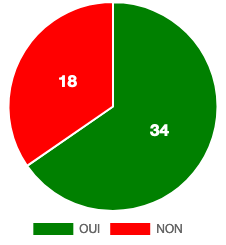
\includegraphics[width=0.69\textwidth]{figures/langueM.png}
        \caption{Réponses à la question : \og Le français est-il votre langue maternelle ?\fg{}}\label{fig:langueM}
    \end{minipage}
    \hfill
    \begin{minipage}[t]{.45\textwidth}
        \centering
        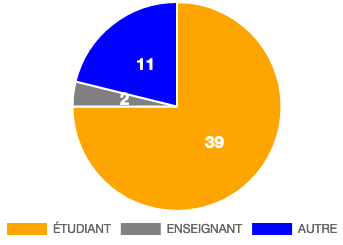
\includegraphics[width=\textwidth]{figures/statut.png}
        \caption{Réponses à la question : \og Quel est votre statut ?\fg{}}\label{fig:statut}
    \end{minipage} 
\end{figure}

\newpage

On constate à travers l'analyse des \textsc{Figs. }\ref{fig:langueM} et \ref{fig:statut} que la majorité des personnes ayant rempli le questionnaire sont des étudiants parlant couramment français. De plus, la plupart des sondés étudient dans le secteur des sciences appliquées (et en particulier en informatique) ce qui est logique étant donné que le lien du formulaire a été diffusé à des étudiants en informatique (voir \textsc{Fig. }\ref{fig:secteur}).

\vspace{5px}

\begin{figure}[htbp]
\begin{center}
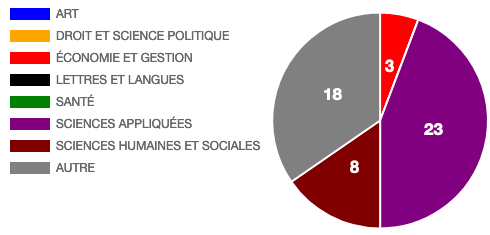
\includegraphics[width=0.65\textwidth]{figures/secteur.png}
\caption{Réponses à la question : \og Quel est votre secteur d'activité ou d'étude ?\fg{}}
\label{fig:secteur}
\end{center}
\end{figure}

\vspace{-15px}

\section{Résultats de l'étude}

\subsection{Sens donné aux propositions}

On constate on observant la \textsc{Fig. }\ref{fig:nb-type} que le nombre de OUI, NON et PEUT-ÊTRE sont à peu près les mêmes laissant suggérer qu'aucun de ces moyens de notation ne semble être privilégié par les utilisateurs. D'autre part, on constate que le temps moyen de réflexion lorsque le sondé répond PEUT-ÊTRE est de 8,9 secondes alors qu'il est seulement de 7,3 secondes quand il répond NON et 6,1 secondes quand il répond OUI (\textsc{Fig. }\ref{fig:temps-type}). On peut donc conclure que le temps de réflexion est plus long quand l'utilisateur répond PEUT-ÊTRE, démontrant que celui-ci hésite longtemps avant de le sélectionner. Les propositions comptant un grand nombre de PEUT-ÊTRE peuvent donc être qualifiées comme très ambiguës d'autant plus que le temps de réflexion y est important.

\vspace{6px}

\begin{figure}[htb]
    \begin{minipage}[t]{.45\textwidth}
        \centering
        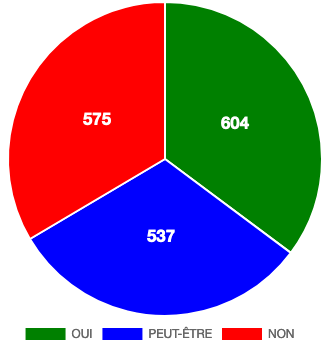
\includegraphics[width=.65\textwidth]{figures/nb-type.png}
        \caption{Nombre de réponse par sens donné aux propositions}\label{fig:nb-type}
    \end{minipage}
    \hfill
    \begin{minipage}[t]{.52\textwidth}
        \centering
        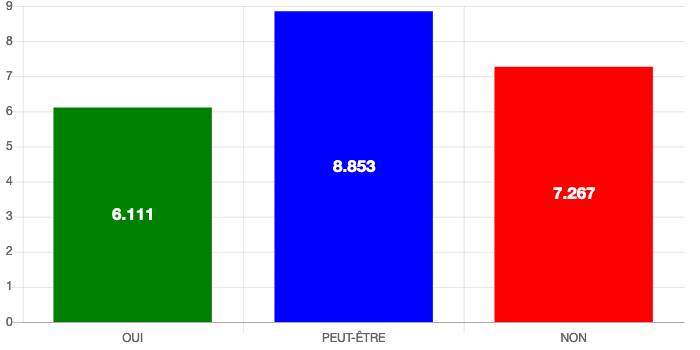
\includegraphics[width=\textwidth]{figures/temps-type.png}
        \caption{Temps de réflexion moyen par sens donné aux propositions (en secondes)}\label{fig:temps-type}
    \end{minipage} 
\end{figure}

\subsection{Ordre des phrases}

On veut démontrer la pertinence de l'aléatoirisation de l'ordre des phrases. On constate avec les résultats rassemblés dans la \textsc{Fig. }\ref{fig:temps-ordre} que les phrases ont un temps de réflexion associé (de lecture de la question et de notation des propositions) plus important quand elles sont abordées au début du questionnaire qu'à la fin. Ce temps de réflexion est globalement décroissant au fur et à mesure que l'on avance dans le questionnaire. L'intérêt d'aléatoiriser l'ordre des phrases est donc essentiel pour garantir la validité des résultats. La variable du temps de réflexion peut donc être exploitée avec un grand nombre de données collectées car chaque sondé aura certes les mêmes phrases mais elles lui seront exposées dans un ordre différent des autres. Dans ce même but de pouvoir exploiter les données de temps de réflexion, nous avons également aléatoirisé l'ordre des propositions pour une même phrase.

\vspace{6px}

\begin{figure}[htbp]
\begin{center}
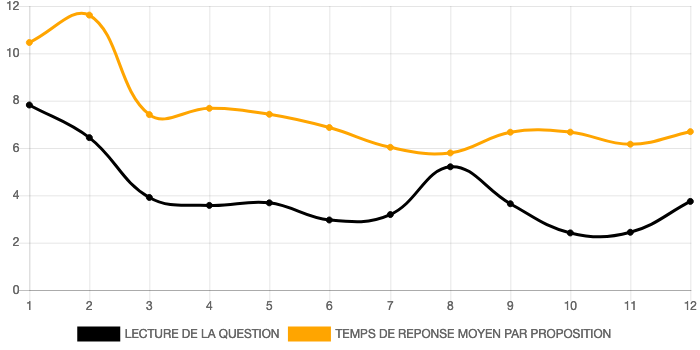
\includegraphics[width=0.85\textwidth]{figures/temps-ordre.png}
\caption{Temps de réflexion moyen par propositions (en secondes) en fonction de l'ordre dans lequel les questions sont abordées}
\label{fig:temps-ordre}
\end{center}
\end{figure}


\subsection{Analyse des résultats}

Nous allons étudier toutes les phrases et les propositions associées à ses phrases en mettant cela en relation avec la \textsc{Fig. }\ref{fig:nb-prop} qui représente la proportion de OUI, NON et PEUT-ÊTRE pour chaque proposition, la \textsc{Fig. }\ref{fig:tab-nb-prop} qui est une simplification de la \textsc{Fig. }\ref{fig:nb-prop} et la \textsc{Fig. }\ref{fig:temps-phrase} qui rassemble les données de temps de réponse pour chaque proposition ainsi que le temps de lecture de la phrase exemple. On peut classer ces phrases en 6 catégories (voir légende de la \textsc{Fig. }\ref{fig:tab-nb-prop}).

\subsubsection{Catégorie n\degres1 - \og OUI \fg{} majoritaire}

Les propositions pour lesquelles le nombre de sondé ayant répondu OUI est majoritaire induit que cette proposition a le même sens que la phrase exemple selon la majorité des sondés. On peut par exemple citer la P4.1\footnote{Px.y désigne la proposition y de la phrase n\degres x} pour laquelle il est vrai selon les sondés d'interpréter \og Un bus ramènera tous les invités \fg{} comme \og Un bus pour tous les invités \fg{}. Il est évident ici qu'il y a un seul bus et que tous les invités montent dans le même. On peut également citer la P2.3 qui est majoritairement notée comme étant vraie. En effet, la phrase \og Toutes les écoles sont fermées un certain jour. \fg{} et la proposition P2.3 \og Toutes les écoles sont fermées un jour (pas forcément différent des autres). \fg{} met en avant l'ambiguïté du quantificateur \og certain \fg{} en disant que des écoles ferment le même jour et d'autres pas. Le sondés notent majoritairement cette proposition comme étant vraie car elle englobe toutes les possibilités liées à cette ambiguïté.\\

On constate que les temps de réponse à la P4.1 et la P2.3 sont respectivement de 4,965 secondes et de 7,65 secondes, ce qui est plutôt rapide quand on compare cela aux autres temps de réponse. La \textsc{Fig. }\ref{fig:temps-type} montre également que le temps de réflexion moyen lorsque le sens de la proposition est OUI est inférieur aux autres : il est de 6,111 secondes alors qu'il est de 8,853 secondes pour PEUT-ÊTRE et 7,267 secondes pour NON.

\vspace{7px}

\subsubsection{Catégorie n\degres2 - \og NON \fg{} majoritaire}

Il y a des propositions pour lesquelles les sondés ont majoritairement répondu NON. C'est le cas pour la P4.2 et la P4.3 correspondant à la phrase 4 \og Un bus ramènera les invités. \fg{}. Dans les deux cas, la proposition est absurde. La P4.2 \og Un bus pour chaque invité. \fg{} sous-entend que chaque invité sera ramené par un bus et qu'il sera le seul dedans, si on suit la logique il faudra autant de bus que d'invités. Pour la P4.3 \og Un même invité dans tous les bus. \fg{}, il s'agit d'une phrase test totalement absurde pour vérifier que les sondés ne répondent pas n'importe quoi. C'est également le cas pour la P5.2 \og Les enfants n’ont pas eu de cadeau. \fg{} de la phrase exemple \og Les enfants ont reçu un cadeau lors du dernier jour d’école. \fg{}. Malgré le fait que certains sondés répondent OUI ou PEUT-ÊTRE à ces propositions car ils ont sans doute mal lu les consignes ou les phrases, on constate que la très grande majorité des personnes répondent NON. Ces phrases là ne sont donc pas ambiguës.\\

\vspace{3px}

\begin{figure}[htbp]
\begin{center}
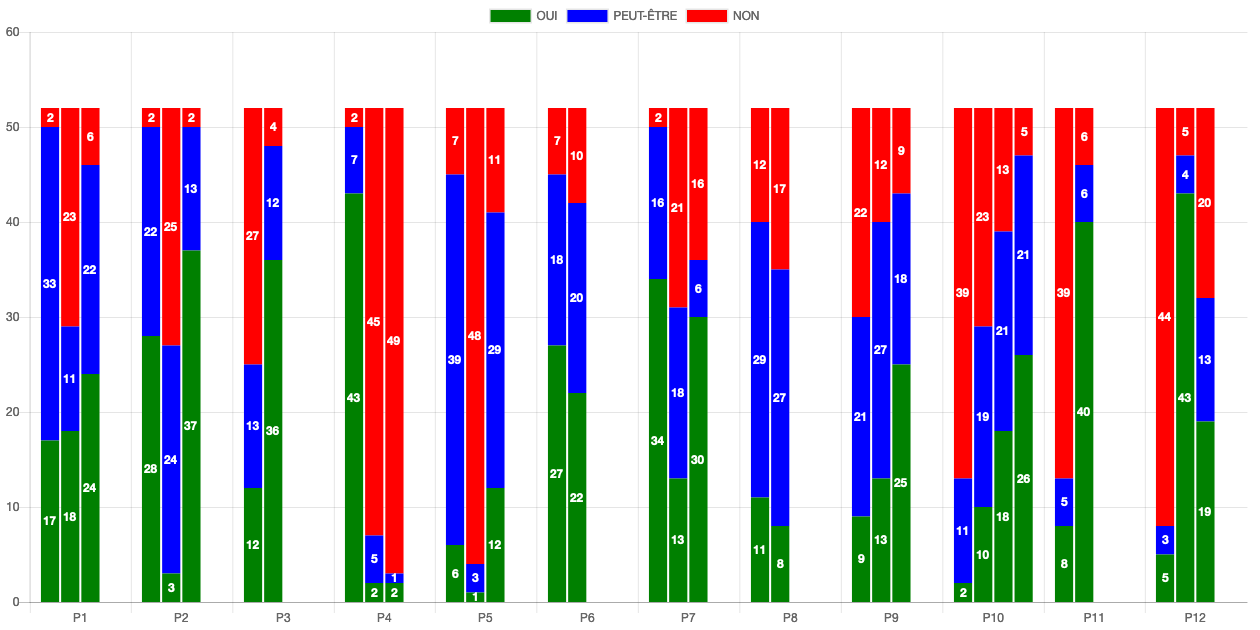
\includegraphics[width=\textwidth]{figures/nb-prop.png}
\caption{Nombre et type de note attribué aux propositions selon le critère : \og Les propositions ont-elles le même sens que la phrase exemple ? \fg{}}
\label{fig:nb-prop}
\end{center}
\end{figure}

Le temps de réflexion associé à la P4.2 est de 7,65 secondes, celui de la P4.3 est de 9,269 secondes et celui de la P5.2 est de 4,634 secondes. En moyenne, ces propositions notées NON sont évaluées une seconde plus lentement que les propositions notées OUI (voir \textsc{Fig. }\ref{fig:temps-type}). On peut interpréter cette différence de temps de réflexion par le fait que certaines propositions sont tellement absurdes et que le sondé se sent obligé de relire les phrases avant de finalement répondre NON car cela n'a effectivement aucun sens.

\vspace{7px}

\subsubsection{Catégorie n\degres3 - \og PEUT-ÊTRE \fg{} majoritaire}

Certaines propositions ont été évaluées majoritairement comme étant ambiguës si bien que les sondés n'ont pas pu dire OUI ou NON, ils ont donc répondu PEUT-ÊTRE. C'est le cas pour la phrase 8 \og Des crayons gratuits seront distribués aux adhérents. \fg{} et les propositions P8.1 \og Chaque adhérent aura droit à maximum un crayon. \fg{} et P8.2 \og Les adhérents auront droit à autant de crayons qu’ils le souhaitent. \fg{}. La phrase exemple 8 ne permet pas de conclure sur le nombre maximum de crayons auquel un adhérent a droit. Pour la phrase 5 \og Les enfants ont reçu un cadeau lors du dernier jour d’école. \fg{} et les propositions P5.1 \og Chaque enfant a reçu un cadeau différent. \fg{} et P5.3 \og Tous les enfants ont reçu le même cadeau. \fg{}, les sondés ont préféré répondre PEUT-ÊTRE pour les mêmes raisons. Cependant, pour la P5.3, une dizaine de personnes sont convaincues que OUI et une autre dizaine que NON. On peut donc qualifier ces phrases d'ambiguës mais les sondés en ont majoritairement conscience car ils répondent PEUT-ÊTRE.\\

Comme on peut le constater avec le graphe de la \textsc{Fig. }\ref{fig:temps-phrase}, le temps de réflexion associé au propositions P8.1, P8.2, P5.1 et P5.3 sont respectivement de 7,33 secondes, 7,894 secondes, 5,523 seconde et 4,266 secondes. D'après la \textsc{Fig. }\ref{fig:temps-type}, lorsque le sondé prend en moyenne 8,853 secondes de réflexion avant de répondre PEUT-ÊTRE, cela ne peut qu'appuyer l'ambiguïté de la phrase. On notera également que la proposition P9.2 \og Tous les musées de la ville ferment le ou les même jours. \fg{} de la phrase 9 \og Tous les musées de la ville ferment certains jours de la semaine. \fg{} atteint un temps de réponse moyen de 21.043 secondes et qu'il s'agit d'une proposition majoritairement notée PEUT-ÊTRE. Cela dénote que la proposition P9.2 soulevait elle-même une ambiguïté en plus de celle apportée par la phrase exemple 9. Nous en arrivons donc à la conclusion que cette proposition a mal été choisie et nous la corrigerons dans la prochaine version du questionnaire.

\vspace{13px}

\begin{figure}[htbp]
\begin{center}
\bgroup
\def\arraystretch{1.5}
\setlength{\tabcolsep}{0.1em}
\begin{tabular}{|c|c|c|c|c|c|c|c|c|c|c|c|c|c|c|c|c|c|c|c|c|c|c|c|c|c|c|c|c|c|c|c|c|}
    \hline
     \multicolumn{3}{|c|}{\textbf{P1}} & \multicolumn{3}{|c|}{\textbf{P2}} & \multicolumn{2}{|c|}{\textbf{P3}} & \multicolumn{3}{|c|}{\textbf{P4}} & \multicolumn{3}{|c|}{\textbf{P5}} & \multicolumn{2}{|c|}{\textbf{P6}} & \multicolumn{3}{|c|}{\textbf{P7}} & \multicolumn{2}{|c|}{\textbf{P8}} & \multicolumn{3}{|c|}{\textbf{P9}} & \multicolumn{4}{|c|}{\textbf{P10}} & \multicolumn{2}{|c|}{\textbf{P11}} & \multicolumn{3}{|c|}{\textbf{P12}}\\
      \hline
      1 & 2 & 3 & 1 & 2 & 3 & 1 & 2 & 1 & 2 & 3 & 1 & 2 & 3 & 1 & 2 & 1 & 2 & 3 & 1 & 2 & 1 & 2 & 3 & 1 & 2 & 3 & 4 & 1 & 2 & 1 & 2 & 3\\
      \hline
      \cellcolor{blue} & \cellcolor{red}\color{white}\textbf{23} & \cellcolor{green}\color{white}\textbf{24} & \cellcolor{green}\color{white}\textbf{28} & \cellcolor{red}\color{white}\textbf{25} & \cellcolor{green} & \cellcolor{red}\color{white}\textbf{27} & \cellcolor{green} & \cellcolor{green} & \cellcolor{red} & \cellcolor{red} & \cellcolor{blue} & \cellcolor{red} & \cellcolor{blue} & \cellcolor{green}\color{white}\textbf{27} & \cellcolor{green}\color{white}\textbf{22} & \cellcolor{green} & \cellcolor{red}\color{white}\textbf{21} & \cellcolor{green} & \cellcolor{blue} & \cellcolor{blue} & \cellcolor{red}\color{white}\textbf{22} & \cellcolor{blue} & \cellcolor{green}\color{white}\textbf{25} & \cellcolor{red} & \cellcolor{red}\color{white}\textbf{23} & \cellcolor{blue}\color{white}\textbf{21} & \cellcolor{green}\color{white}\textbf{26} & \cellcolor{red} & \cellcolor{green} & \cellcolor{red} & \cellcolor{green} & \cellcolor{red}\color{white}\textbf{20}\\
      
      \multirow{-2}{*}{\cellcolor{blue}\color{white}\textbf{33}} & \cellcolor{green}\color{white}\textbf{18} & \cellcolor{blue}\color{white}\textbf{22} & \cellcolor{blue}\color{white}\textbf{22} & \cellcolor{blue}\color{white}\textbf{24} & \multirow{-2}{*}{\cellcolor{green}\color{white}\textbf{37}} & \cellcolor{blue}\color{white}\textbf{13} & \multirow{-2}{*}{\cellcolor{green}\color{white}\textbf{36}} & \multirow{-2}{*}{\cellcolor{green}\color{white}\textbf{43}} & \multirow{-2}{*}{\cellcolor{red}\color{white}\textbf{45}} & \multirow{-2}{*}{\cellcolor{red}\color{white}\textbf{49}} & \multirow{-2}{*}{\cellcolor{blue}\color{white}\textbf{39}} & \multirow{-2}{*}{\cellcolor{red}\color{white}\textbf{48}} & \multirow{-2}{*}{\cellcolor{blue}\color{white}\textbf{29}} & \cellcolor{blue}\color{white}\textbf{18} & \cellcolor{blue}\color{white}\textbf{20} & \multirow{-2}{*}{\cellcolor{green}\color{white}\textbf{34}} & \cellcolor{blue}\color{white}\textbf{18} & \multirow{-2}{*}{\cellcolor{green}\color{white}\textbf{30}} & \multirow{-2}{*}{\cellcolor{blue}\color{white}\textbf{29}} & \multirow{-2}{*}{\cellcolor{blue}\color{white}\textbf{27}} & \cellcolor{blue}\color{white}\textbf{21} & \multirow{-2}{*}{\cellcolor{blue}\color{white}\textbf{27}} & \cellcolor{blue}\color{white}\textbf{18} & \multirow{-2}{*}{\cellcolor{red}\color{white}\textbf{39}} & \cellcolor{blue}\color{white}\textbf{19} & \cellcolor{green}\color{white}\textbf{16} & \cellcolor{blue}\color{white}\textbf{21} & \multirow{-2}{*}{\cellcolor{red}\color{white}\textbf{39}} & \multirow{-2}{*}{\cellcolor{green}\color{white}\textbf{40}} & \multirow{-2}{*}{\cellcolor{red}\color{white}\textbf{44}} & \multirow{-2}{*}{\cellcolor{green}\color{white}\textbf{43}} & \cellcolor{blue}\color{white}\textbf{19}\\
      \hline
\end{tabular}
\egroup

\vspace{10px}

\begin{tabular}{|cc|l|l|}
    \hline
      \cellcolor{green} & \cellcolor{green} & OUI majoritaire & Proposition vraie selon la majorité des sondés\\
      \hline
      \cellcolor{red} & \cellcolor{red} & NON majoritaire & Proposition fausse ou incohérente selon la majorité des sondés\\
      \hline
      \cellcolor{blue} & \cellcolor{blue} & PEUT-ÊTRE majoritaire & Proposition ambiguë mais le sondé en a conscience \\
      \hline
      \cellcolor{green} & \cellcolor{blue} & OUI et PEUT-ÊTRE majoritaires & Proposition ambiguë mais plutôt vraie \\
      \hline
      \cellcolor{red} & \cellcolor{blue} & NON et PEUT-ÊTRE majoritaires & Proposition ambiguë mais plutôt fausse \\
      \hline
      \cellcolor{green} & \cellcolor{red} & OUI et NON majoritaires & Proposition ambiguë et interprétée différemment selon les sondés \\
      \hline
\end{tabular}
\caption{Interprétation et simplification de la \textsc{Fig. }\ref{fig:nb-prop} avec la mise en avant de la/des note(s) majoritaire(s) pour chaque proposition}
\label{fig:tab-nb-prop}
\end{center}
\end{figure}

\subsubsection{Catégorie n\degres4 - \og OUI \fg{} et \og PEUT-ÊTRE \fg{} majoritaires}

Les propositions répondant à ce critère sont considérées comme ambiguës en pleine conscience par certains sondés (ceux qui répondent PEUT-ÊTRE) et sont vraies pour d'autres (ceux qui répondent OUI). Certaines personnes y voient donc différents sens possibles alors que d'autres sont convaincues que c'est vrai et n'y voient pas une potentielle ambiguïté. Parmi ces propositions, on peut citer la P6.1 \og Certaines entreprises vont faire faillite. \fg{} et la P6.2 \og Toutes les entreprises vont faire faillite. \fg{} de la phrase 6 \og Les entreprises vont faire faillite. \fg{}.

\subsubsection{Catégorie n\degres5 - \og NON \fg{} et \og PEUT-ÊTRE \fg{} majoritaires}

A l'inverse, certaines propositions comme la P10.2 \og Tous les étudiants cherchent un travail différent. \fg{} de la phrase 10 \og Des étudiants cherchent du travail. \fg{} ont un nombre de NON et de PEUT-ÊTRE élevé. Certains sondés voient l'ambiguïté de \og Des \fg{} alors que d'autres sont convaincus que \og Des \fg{} veut dire \og Tous \fg{} dans ce cas là.

\vspace{7px}

\begin{figure}[htbp]
\begin{center}
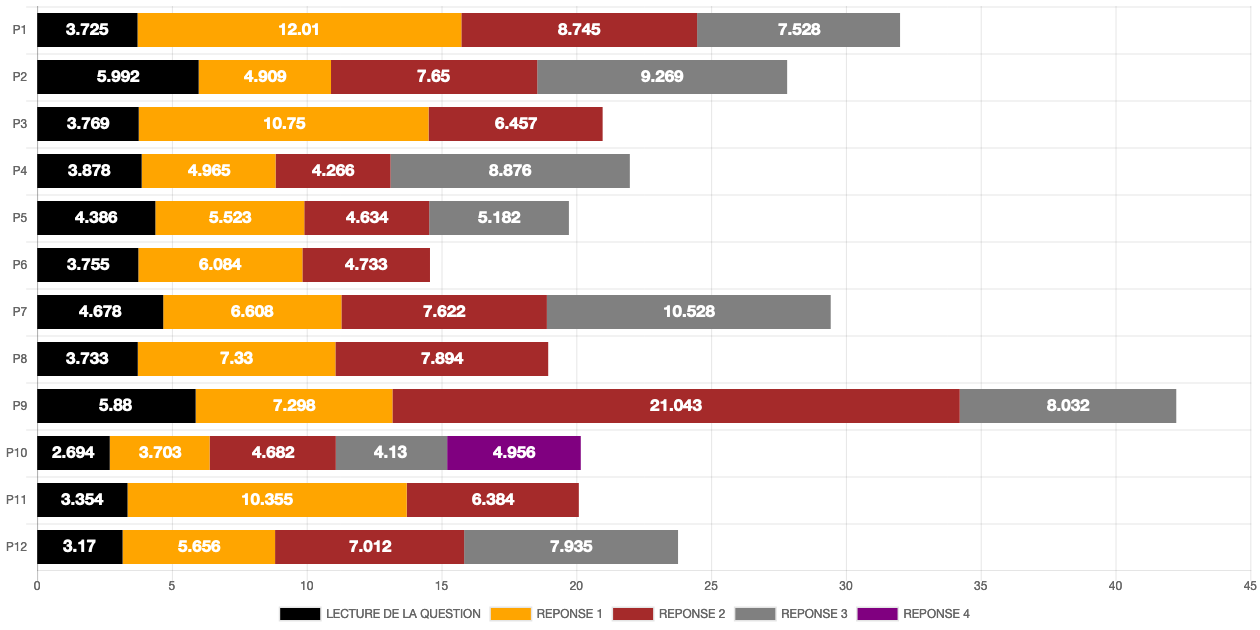
\includegraphics[width=\textwidth]{figures/temps-phrase.png}
\caption{Temps de réflexion moyen par phrase (en secondes)}
\label{fig:temps-phrase}
\end{center}
\end{figure}

\vspace{-20px}

\subsubsection{Catégorie n\degres6 - \og OUI \fg{} et \og NON \fg{} majoritaires}

Sur les 33 propositions du questionnaire, une seule répond à ce critère. Il s'agit de la P1.2 \og Un gardien différent doit surveiller la salle qui lui a été assignée. \fg{} de la phrase 1 \og Un gardien surveille chaque salle du musée. \fg{}. Cette proposition est interprétée différemment selon les sondés. Ceux qui répondent OUI considèrent que chaque gardien surveille une salle différente et que celle-ci lui a été assignée. Ceux qui répondent NON considèrent que surveiller \og chaque salle \fg{} ne restreint pas la surveillance qu'à une seule. Il n'y a pas de bonne ou de mauvaise réponse  ici et comme dans tout le questionnaire. Dans ce cas là cependant, il y a une grosse différence d'interprétation sans que le sondé en ai conscience. Le temps de réflexion associé à cette proposition est de 8,745 secondes, ce qui est dans la moyenne des phrases à laquelle les sondés répondent majoritairement PEUT-ÊTRE. Avant de répondre à cette question la personne hésite longtemps sans pour autant répondre PEUT-ÊTRE. Cette phrase est donc très ambiguë mais le sondé donne plutôt un avis tranché à la fin.

\newpage

\subsection{Interprétation de \og les \fg{} et \og des \fg{}}

Quelques données à propos de l'interprétation des mots \og les \fg{} et \og des \fg{} par les sondés sont rassemblées dans la \textsc{Fig. }\ref{fig:conclusion}. On constate que \og les \fg{} est interprété comme \og tous/toutes \fg{} ou \og certains/certaines \fg{} alors que \og des \fg{} est seulement interprété comme \og certains/certaines \fg{}. En effet, \og L'ensemble F contient des éléments de l'ensemble E.\fg{} sous-entend que l'on ne fait pas référence à tous les éléments de l'ensemble E, mais qu'il peut y avoir au moins un élément de E qui n'est pas dans F.

\vspace{7px}

\begin{figure}[htbp]
\begin{center}
\begin{tabular}{|c|c|c|c|}
    \hline
      \textbf{Mot} & \textbf{Interprétation} & \textbf{Note majoritaire} & \textbf{Phrases}\\
      \hline
      \multirow{3}{*}{Les} & Chaque & \cellcolor{blue} & P5.1\\\cline{2-4}
      & Tous/Toutes & \cellcolor{green} & P5.3, P6.2\\\cline{2-4}
      & Certains/Certaines & \cellcolor{green} & P6.1\\
      \hline
      \multirow{2}{*}{Des} & Tous/Toutes & \cellcolor{red} & P10.1, P10.2\\\cline{2-4}
      & Certains/Certaines & \cellcolor{green} & P10.3, P10.4\\
      \hline
    \end{tabular}
\caption{Interprétation de \og les \fg{} et \og des \fg{} par les sondés}
\label{fig:conclusion}
\end{center}
\end{figure}

Il est difficile de tirer d'autres conclusions sur l'interprétation d'un mot en particulier avec les phrases que nous avons choisies. En effet, le fait de placer plusieurs quantificateurs dans la même phrase rend l'analyse des notations difficiles car on ne sait pas quel(s) quantificateur(s) a/ont fait pencher la balance lorsque le sondé a noté la phrase en question.

\newpage

\setcounter{section}{0}
\part{Perspectives pour le second semestre}

\section{Diversité des phrases}

Afin d'améliorer le questionnaire, nous allons construire automatiquement des phrases ambiguës pour apporter des variations dans le questionnaire. L'idée est de garder quasiment les mêmes 12 squelettes de phrases que l'on a étudié ce semestre et de varier les noms, les verbes, les compléments, les temps des phrases et les quantificateurs. Un des points critique est l'accord des mots de la phrase en fonction des temps et du contexte. Voici un exemple avec la phrase n\degres7 \og Un cercle touche chacun des carrés.\fg{}. On peut faire varier ce qui a été évoqué pour générer des phrases avec le même squelette (voir \textsc{Fig. }\ref{fig:tab}).

\vspace{5px}

\begin{figure}[htbp]
\begin{center}
\begin{tabular}{|c|c|c|c|c|c|}
    \hline
      \textbf{Préposition 1} & \textbf{Nom 1} & \textbf{Verbe} & \textbf{Quantificateur} & \textbf{Préposition 2} & \textbf{Nom 2}\\
      \hline
      Un & cercle & touche & chacun & des & carrés\\
      \hline
      Un & cercle & touche & \textit{tous} & \textit{les} & carrés\\
      \hline
      Un & cercle & touche & \textit{un seul} & des & carrés\\
      \hline
      Un & cercle & \textit{touchera} & chacun & des & carrés\\
      \hline
      \textit{Des} & \textit{cercles} & \textit{touchent} & chacun & des & carrés\\
      \hline
      Un & \textit{triangle} & touche & chacun & des & carrés\\
      \hline
      Un & \textit{chasseur} & \textit{tire sur} & chacun & des & \textit{canards}\\
      \hline
    \end{tabular}
\caption{Exemple de variations avec la phrase n\degres7 \og Un cercle touche chacun des carrés \fg{}}
\label{fig:tab}
\end{center}
\end{figure}

\vspace{-8px}

Afin de réaliser cette génération automatique de phrases, nous comptons rassembler les mots par champ lexical (voir \textsc{Fig. }\ref{fig:tab2}). On peut par exemple former les phrases : \og Un footballeur fait une passe à chacun de ses coéquipiers. \fg{}, \og Les ailiers font des passes à leurs attaquants. \fg{}, \og La patronne salue tous ses collègues. \fg{} ou \og Les ouvriers saluent chacun le président. \fg{}.

\vspace{8px}

\begin{figure}[htbp]
\begin{center}
\begin{tabular}{|c|c|c|c|c|c|}
    \hline
      \textbf{Groupe 1 (touche)} & \textbf{Groupe 2 (tire sur)} & \textbf{Groupe 3  (fait une passe à)} & \textbf{Groupe 4 (salue)}\\
      \hline
      cercle & chasseur & footballeur & collègue\\
      \hline
      triangle & canard & handballeur & patron\\
      \hline
      carré & sanglier & basketteur & patronne\\
      \hline
      losange & lapin & attaquant & ouvrier\\
      \hline
      rectangle & chevreuil & ailier & président\\
      \hline
      droite & lièvre & coéquipier & présidente\\
      \hline
      segment & faisan & gardien & secrétaire\\
      \hline
    \end{tabular}
\caption{Exemple de groupes de mots rassemblés par champ lexical et en lien avec la \textsc{Fig. }\ref{fig:tab}}
\label{fig:tab2}
\end{center}
\end{figure}

\vspace{-25px}

\section{Autres améliorations}

Nous n'avons pas eu le temps de faire l'analyse en fonction de si le français est la langue maternelle du sondé. Il faut également pouvoir diffuser le questionnaire plus largement et à des personnes ayant des secteurs d'activité ou d'étude plus variés. En récoltant ces données, on pourrait alors potentiellement mettre en relation les préférences des locuteurs avec leur secteur d'activité ou d'étude. Enfin, concernant le questionnaire actuel, le renseignement de l'adresse mail n'est pas opérationnel dû à des problèmes de PHP qui n'ont pas pu être résolus. Tout cela peut donc être amélioré dans la prochaine version du questionnaire au second semestre.

\newpage

\part{Annexe}
\setcounter{section}{0}

\section{Compte rendu des réunions}

% Début 14/10/19
\subsection{Lundi 14/10/19}
Mettre les phrases manuellement (faire la génération automatique plus
tard, afin de garder assez de temps pour la diffusion et l'analyse statistique). \vspace{5mm}
    
\textbf{Questionnaire} :
\begin{itemize}
    \item La langue française est-elle votre langue maternelle ?
    \item Quel est votre âge ?
    \item Quel est votre domaine d'étude (et/ou secteur d'activité) ?
\end{itemize} \vspace{5mm}

\textbf{Fin décembre} :
\begin{itemize}
    \item Avoir des pages de questions faites à la main
    \item Avoir une base de données
    \item Avoir un timer (chronométrer le temps de réponse)
\end{itemize} \vspace{5mm}
    
\textbf{Après Noël} : Améliorer
\begin{itemize}
    \item Avoir un vrai accès au site (si on ne l'avait pas avant)
    \item Génération de phrases/questions
\end{itemize} \vspace{5mm}
    
\textbf{Site et Questionnaire} :
\begin{itemize}
    \item Faire la demande pour avoir un serveur accessible depuis l'extérieur
        
    \item Des phrases avec 2 quantificateurs :
    \begin{itemize}
        \item ?? (Pour tout)
        \item Exemples : Tous, Chaque, Les, Tous les, ...
        \item Existentiel (Il existe)
        \item Exemples : Un, Certains, Quelques, ...
        \item Et permuter les quantificateurs de places
    \end{itemize}
    \item Il faut des phrases ambiguës
\end{itemize} \vspace{5mm}

\textbf{Exemples de phrases} :
\begin{itemize}
    \item Les enfants prendront une pizza
    \item Est-ce qu'elle a des enfants ? Oui, un. (On peut vouloir dire 'Pour tout', 'Il existe', '1')
\end{itemize} \vspace{5mm}

Voir l'article d'Arthur Capetier sur ses expériences audios. \vspace{5mm}
% Fin 14/10/19

% Début Jour 04/11/19
\newpage
\subsection{Lundi 04/11/19}

\textbf{Changement sur les phrase}

\begin{itemize}
    \item Mettre la 11ème phrase avec \textit{Tous les touristes}
    \item Mettre la 10ème phrase \textit{Un travail}, la phrase n'est pas très ambiguë.
\end{itemize} 

\vspace{5mm}
\textbf{Écrire des phrases}
\begin{itemize}
    \item Faire varier \textit{Tous les} avec \textit{chaque} ect...
    \item exemple: Les mêmes phrase: \textit{Un étudiant doit avoir sa carte étudiant semble} être équivalent à \textit{Tous les etudiants}
\end{itemize}
Utiliser des quantificateurs comme \textit{UN}, \textit{AU MOINS}... Et des quantificateurs universels \textit{TOUS LES}, \textit{UN}, \textit{LE}.
%Fin Jour 04/11/19

\vspace{5px}

% Début Jour 18/11/19
\subsection{Lundi 18/11/19}

\textbf{Avancement du site Web }
\begin{itemize}
\item Mettre la première question (sur les vidéos surveillences) en dernier. En effet cela semble être une question qui n'a pas beaucoup d'ambiguïté en fonction de l'âge.
\item Ajouter les sections Droit, Santé, Science Humaine, Science, Lettre, Science Eco.
\item Stocker l'ordre des réponses et des questions des utilisateurs et les utiliser pour l'étude statistique.
\item Mettre le timer pour chronométrer les questions.
\item Génération attention des mots
\item  Attention sur la diffusion des résultats, \textit{ne pas parler du résultat des autres mais les résultats par rapport aux autres}.
\end{itemize}
\textbf{Rédaction du compte rendu}
\begin{itemize}
\item Commencer la bibliographie
\item Répartition des tâches, chacun doit prendre un partie et rédiger un plan détaillé.
\item Déroulé du projet, organisation, mettre les statistiques à la fin du projet sur les données saisies du premier site
\item Ajout éventuel d'un diagramme de Gantt.
\end{itemize}
% Fin Jour 18/11/19

\vspace{8px}

% Début Jour 04/12/19
\subsection{Lundi 02/12/19}
Regarder si le choix des mots pour symboliser un quantificateur influence le sens que comprend le locuteur.
\vspace{5mm}
% Fin Jour 04/12/19

\vspace{8px}

% Début Jour 18/12/19
\subsection{Jeudi 18/12/19}
Pour le rapport:
\begin{itemize}
    \item Mettre un diagramme de Gantt
    \item Parler des articles que nous avons lu et analysé
\end{itemize}{} \vspace{5mm}

\newpage

\section{Table Utilisateur - Schéma de la base de données}

\vspace{15px}

\begin{center}
    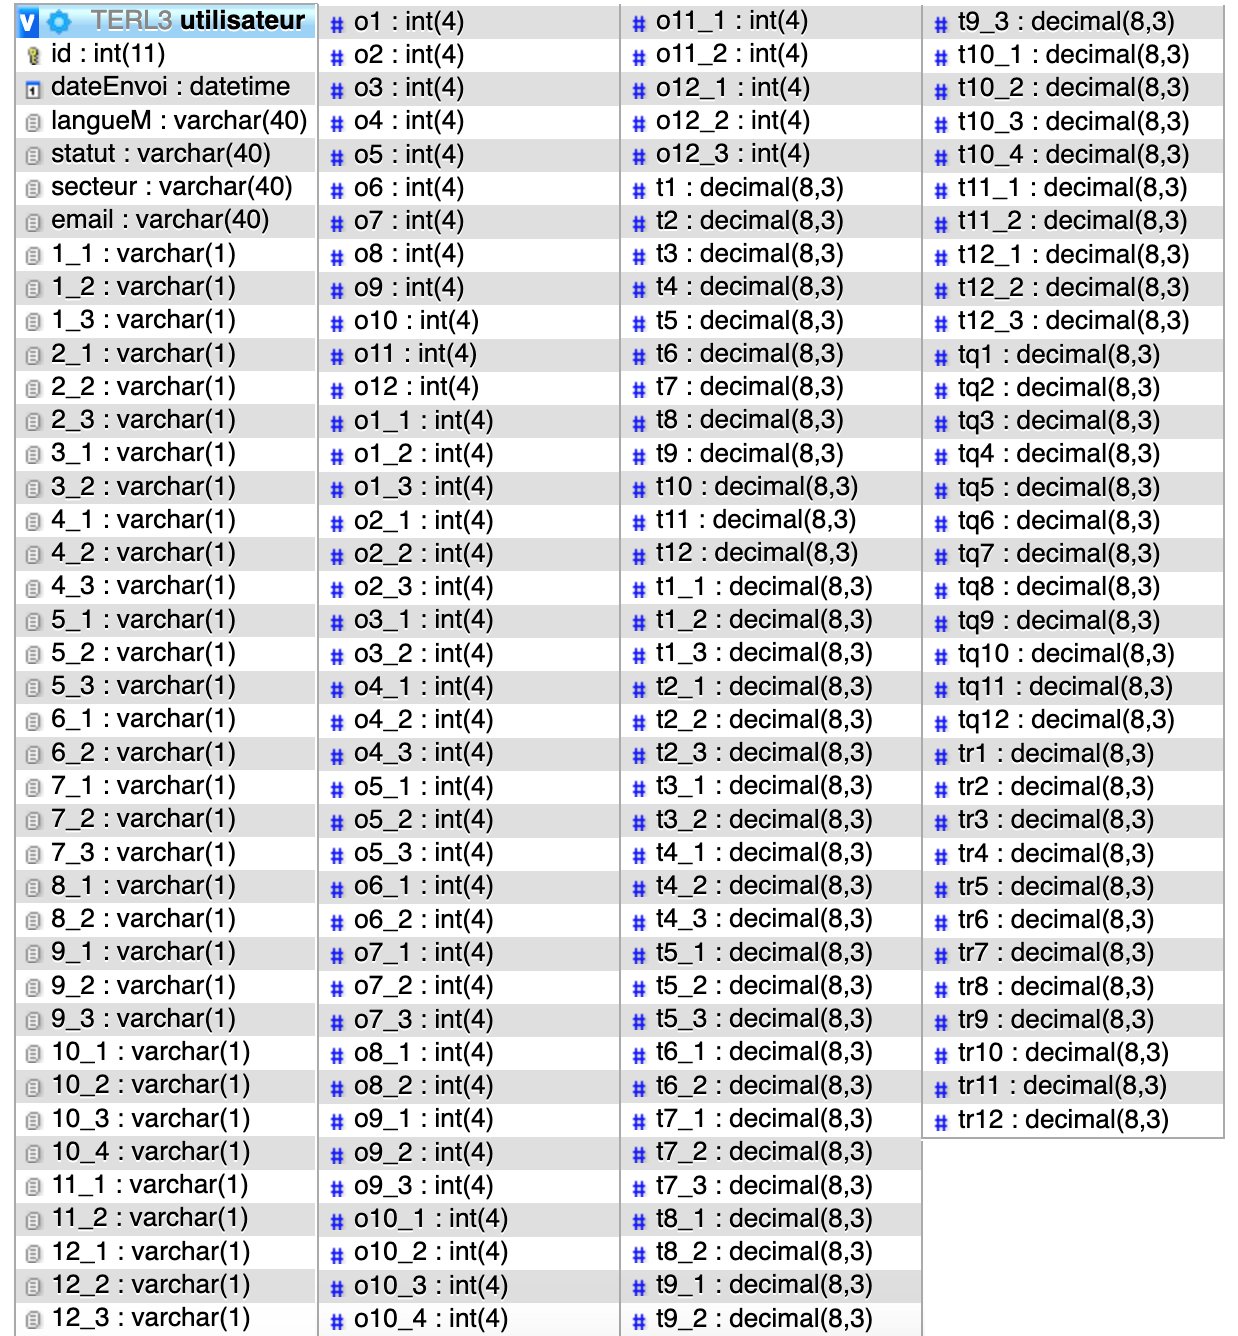
\includegraphics[width=\textwidth]{figures/bdd.png}
\end{center}

\newpage

\section{Données récoltées}

\begin{center}
    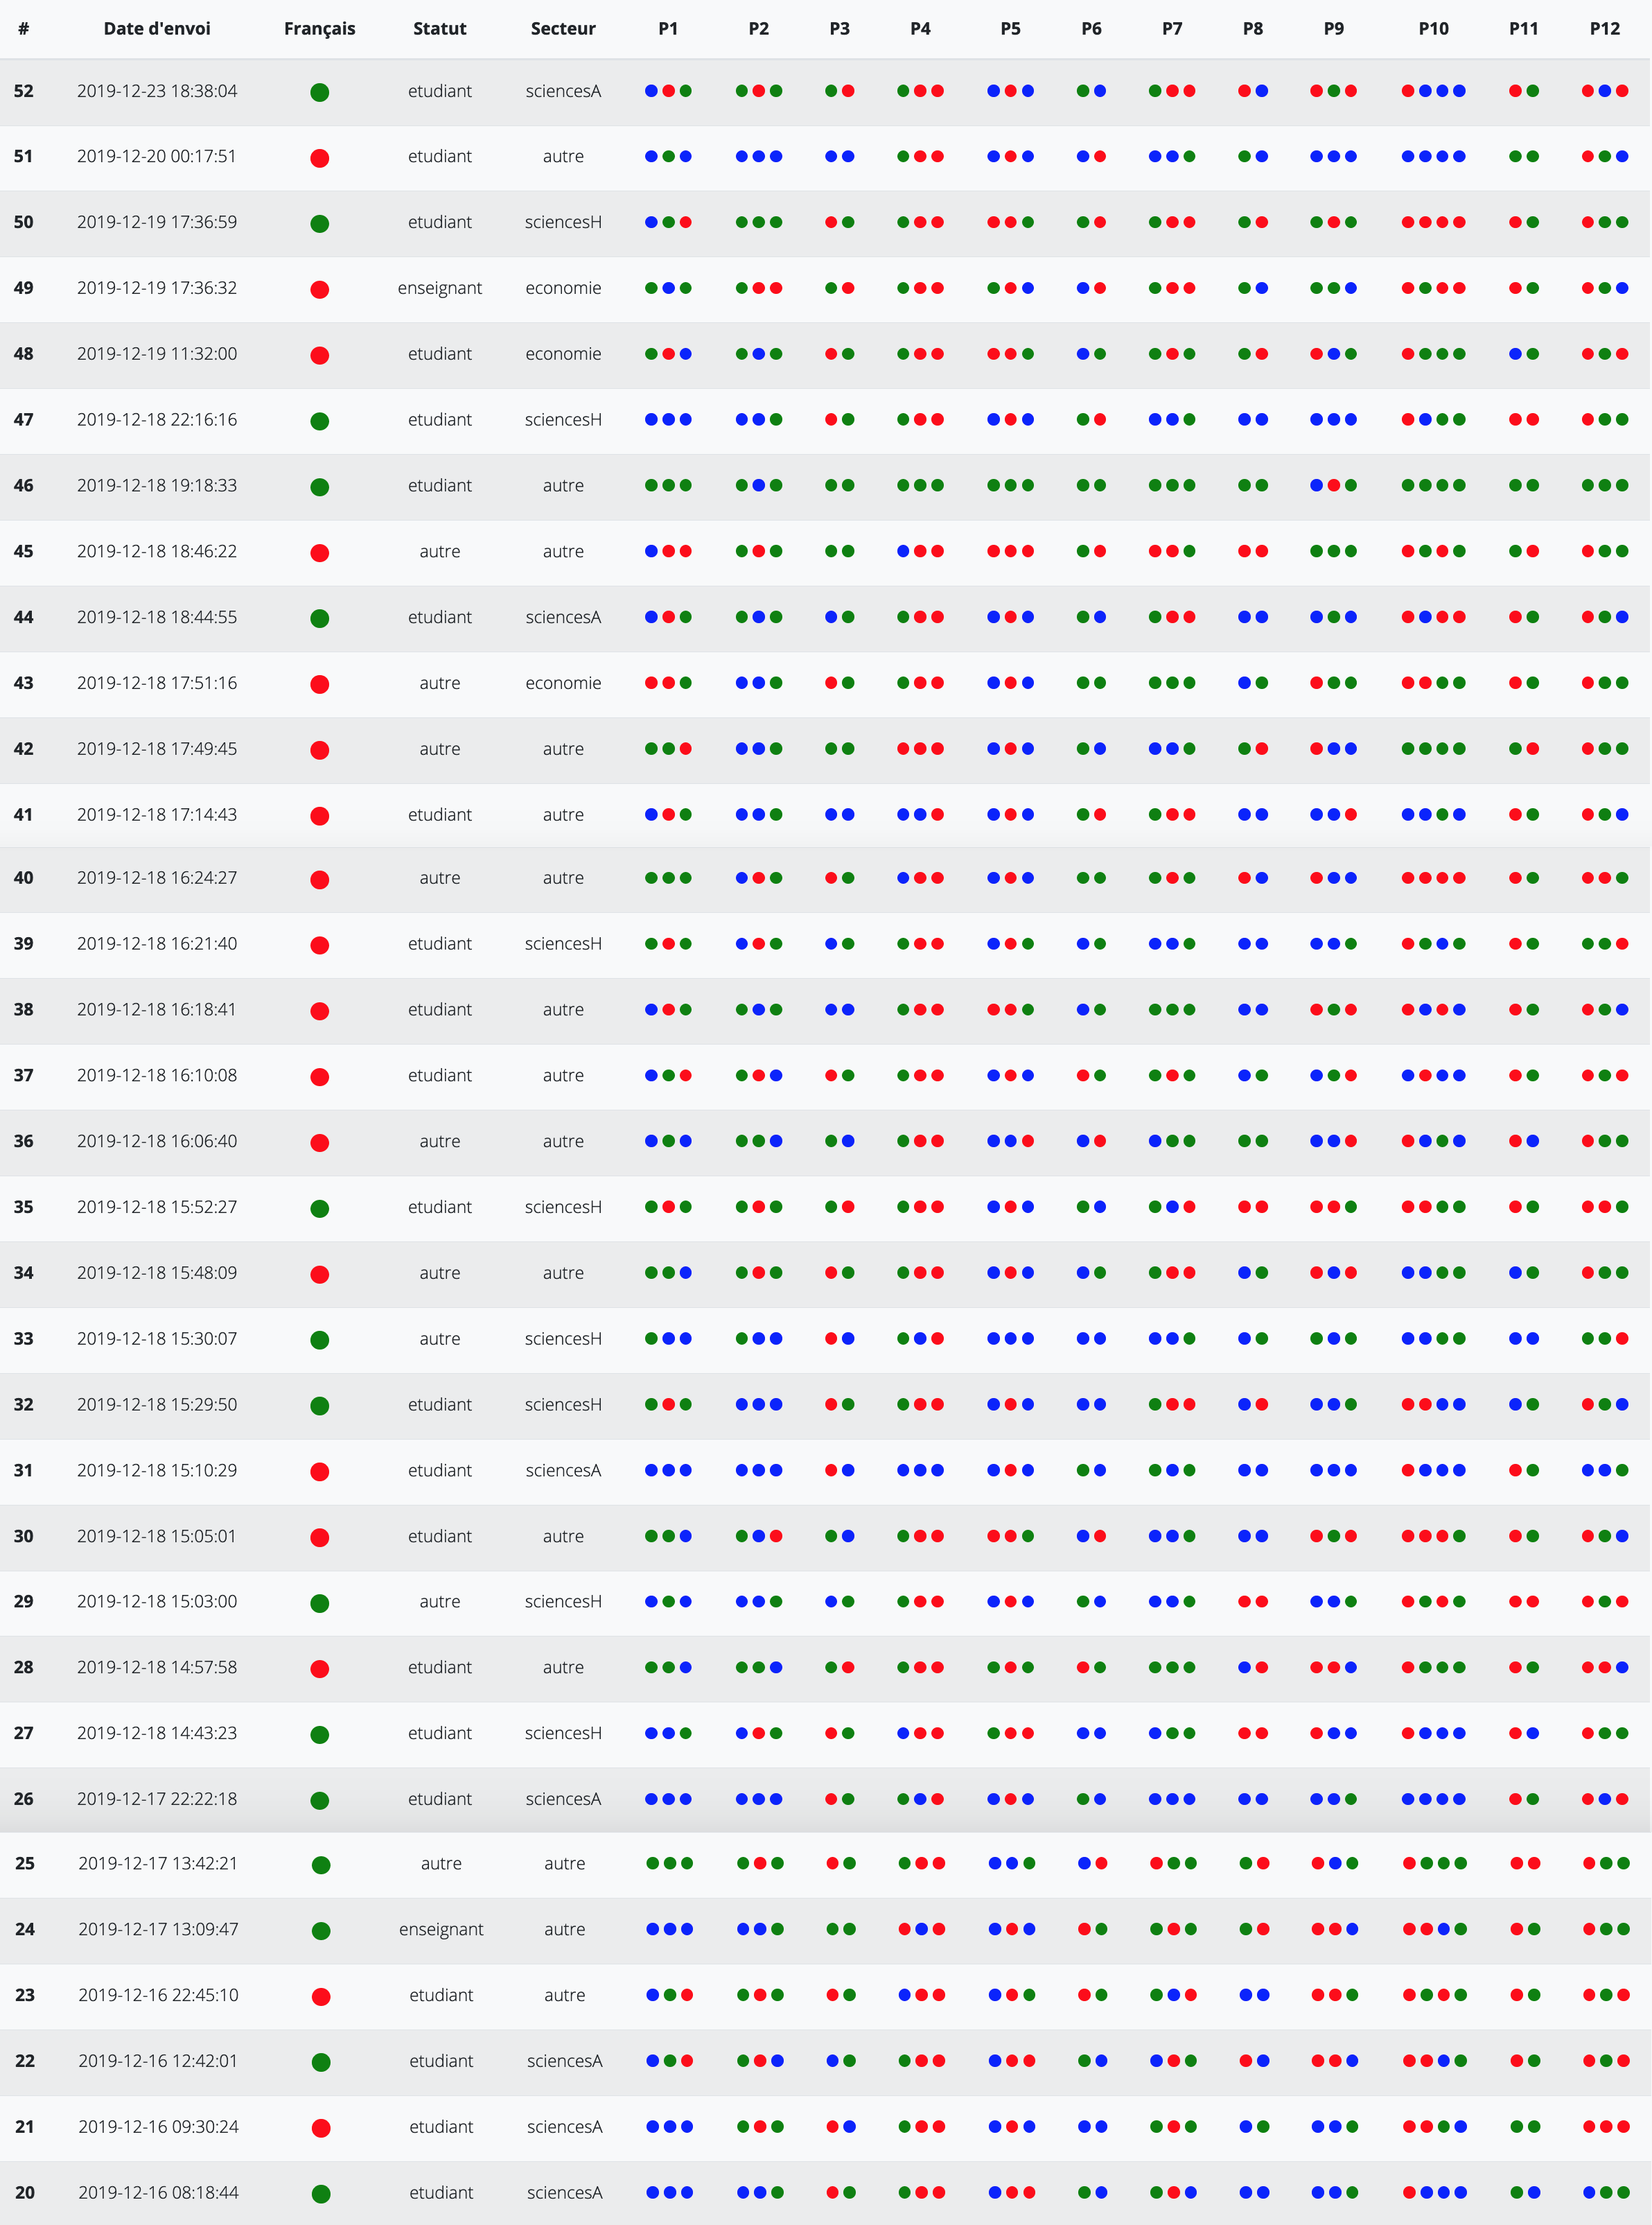
\includegraphics[width=0.9\textwidth]{figures/reponses.png}
\end{center}

\newpage

\begin{center}
    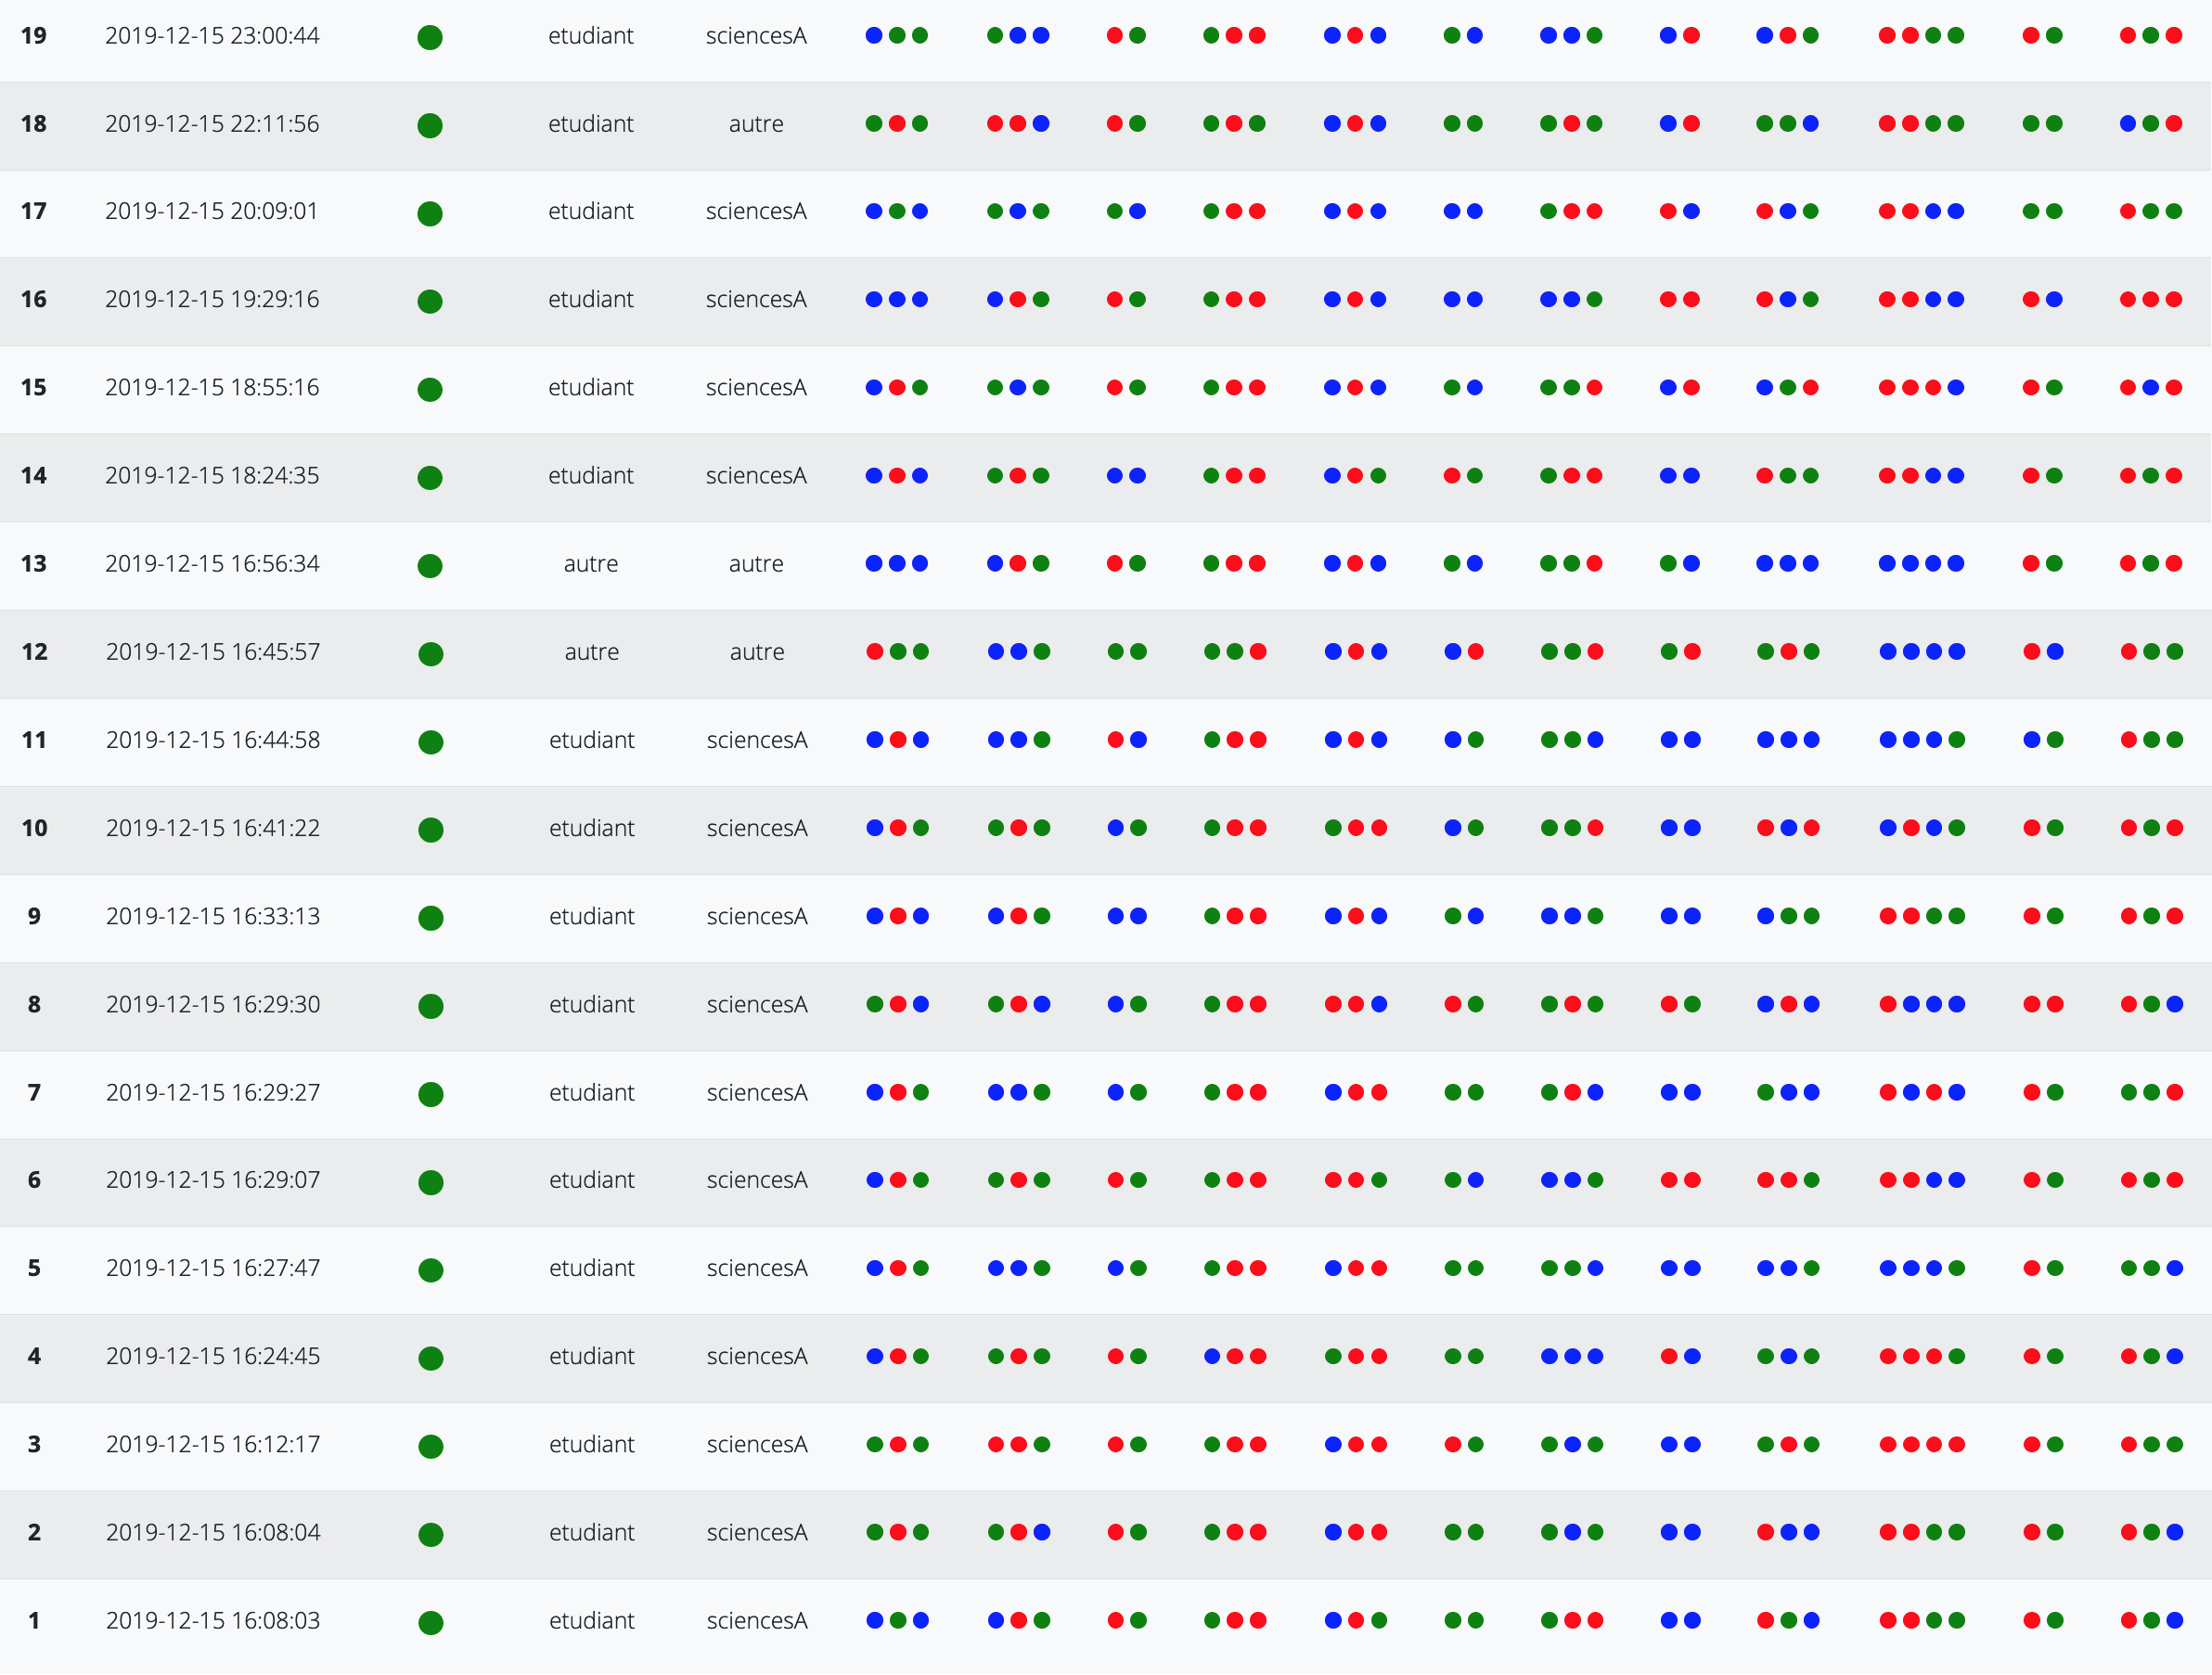
\includegraphics[width=\textwidth]{figures/reponses2.png}
\end{center}

\bibliographystyle{plain}
\bibliography{biblio}

\end{document}